\chapter{Electromagnetic Damping}

\section*{Objectives}

\begin{enumerate}
\itemsep0em
\item To study the generation of eddy currents in a moving conductor.
\item To study the effects of electromagnetic damping on a rotating flywheel.
\end{enumerate}



\section*{Introduction}

In this experiment, you will study the effects of electromagnetic damping on a metal disc in an external magnetic field. When a conductor moves in a magnetic field -- or when a magnetic field varies across a conductor -- an electromotive force is induced which causes loops of current to flow in the conductor. Currents set up like this in conductors are called \textsl{eddy} currents, in analogy to the eddies and vortices seen in the flow of turbulent fluids. 

These induced eddy currents create their own magnetic field that opposes the change in the magnetic field that created it, and this -- as you will see below -- results in an overall damping force on the motion of the conductor. Thus, despite the fact that the disc is non-magnetic, it experiences a retarding force purely due to the fact that it is made of a conductive material. Such a phenomenon is known as \textsl{electromagnetic damping}.

In this experiment, you will study the phenomenon of electromagnetic damping in a rotating aluminium disk. The disc is mounted on a horizontal axle around which a cord is wound, as shown in Figure~(\ref{fig:emdamping-setup}). This cord is in turn attached to a slotted mass, which is allowed to fall, rotating the disc in the process. Two magnets are placed on either side of the disc, which produce the external magnetic field that causes the disc to slow down until it rotates at a constant angular velocity. In turn, the slotted mass stops accelerating downwards, and begins to move at a constant ``terminal'' velocity.

\begin{figure}[!htb]
    \centering
    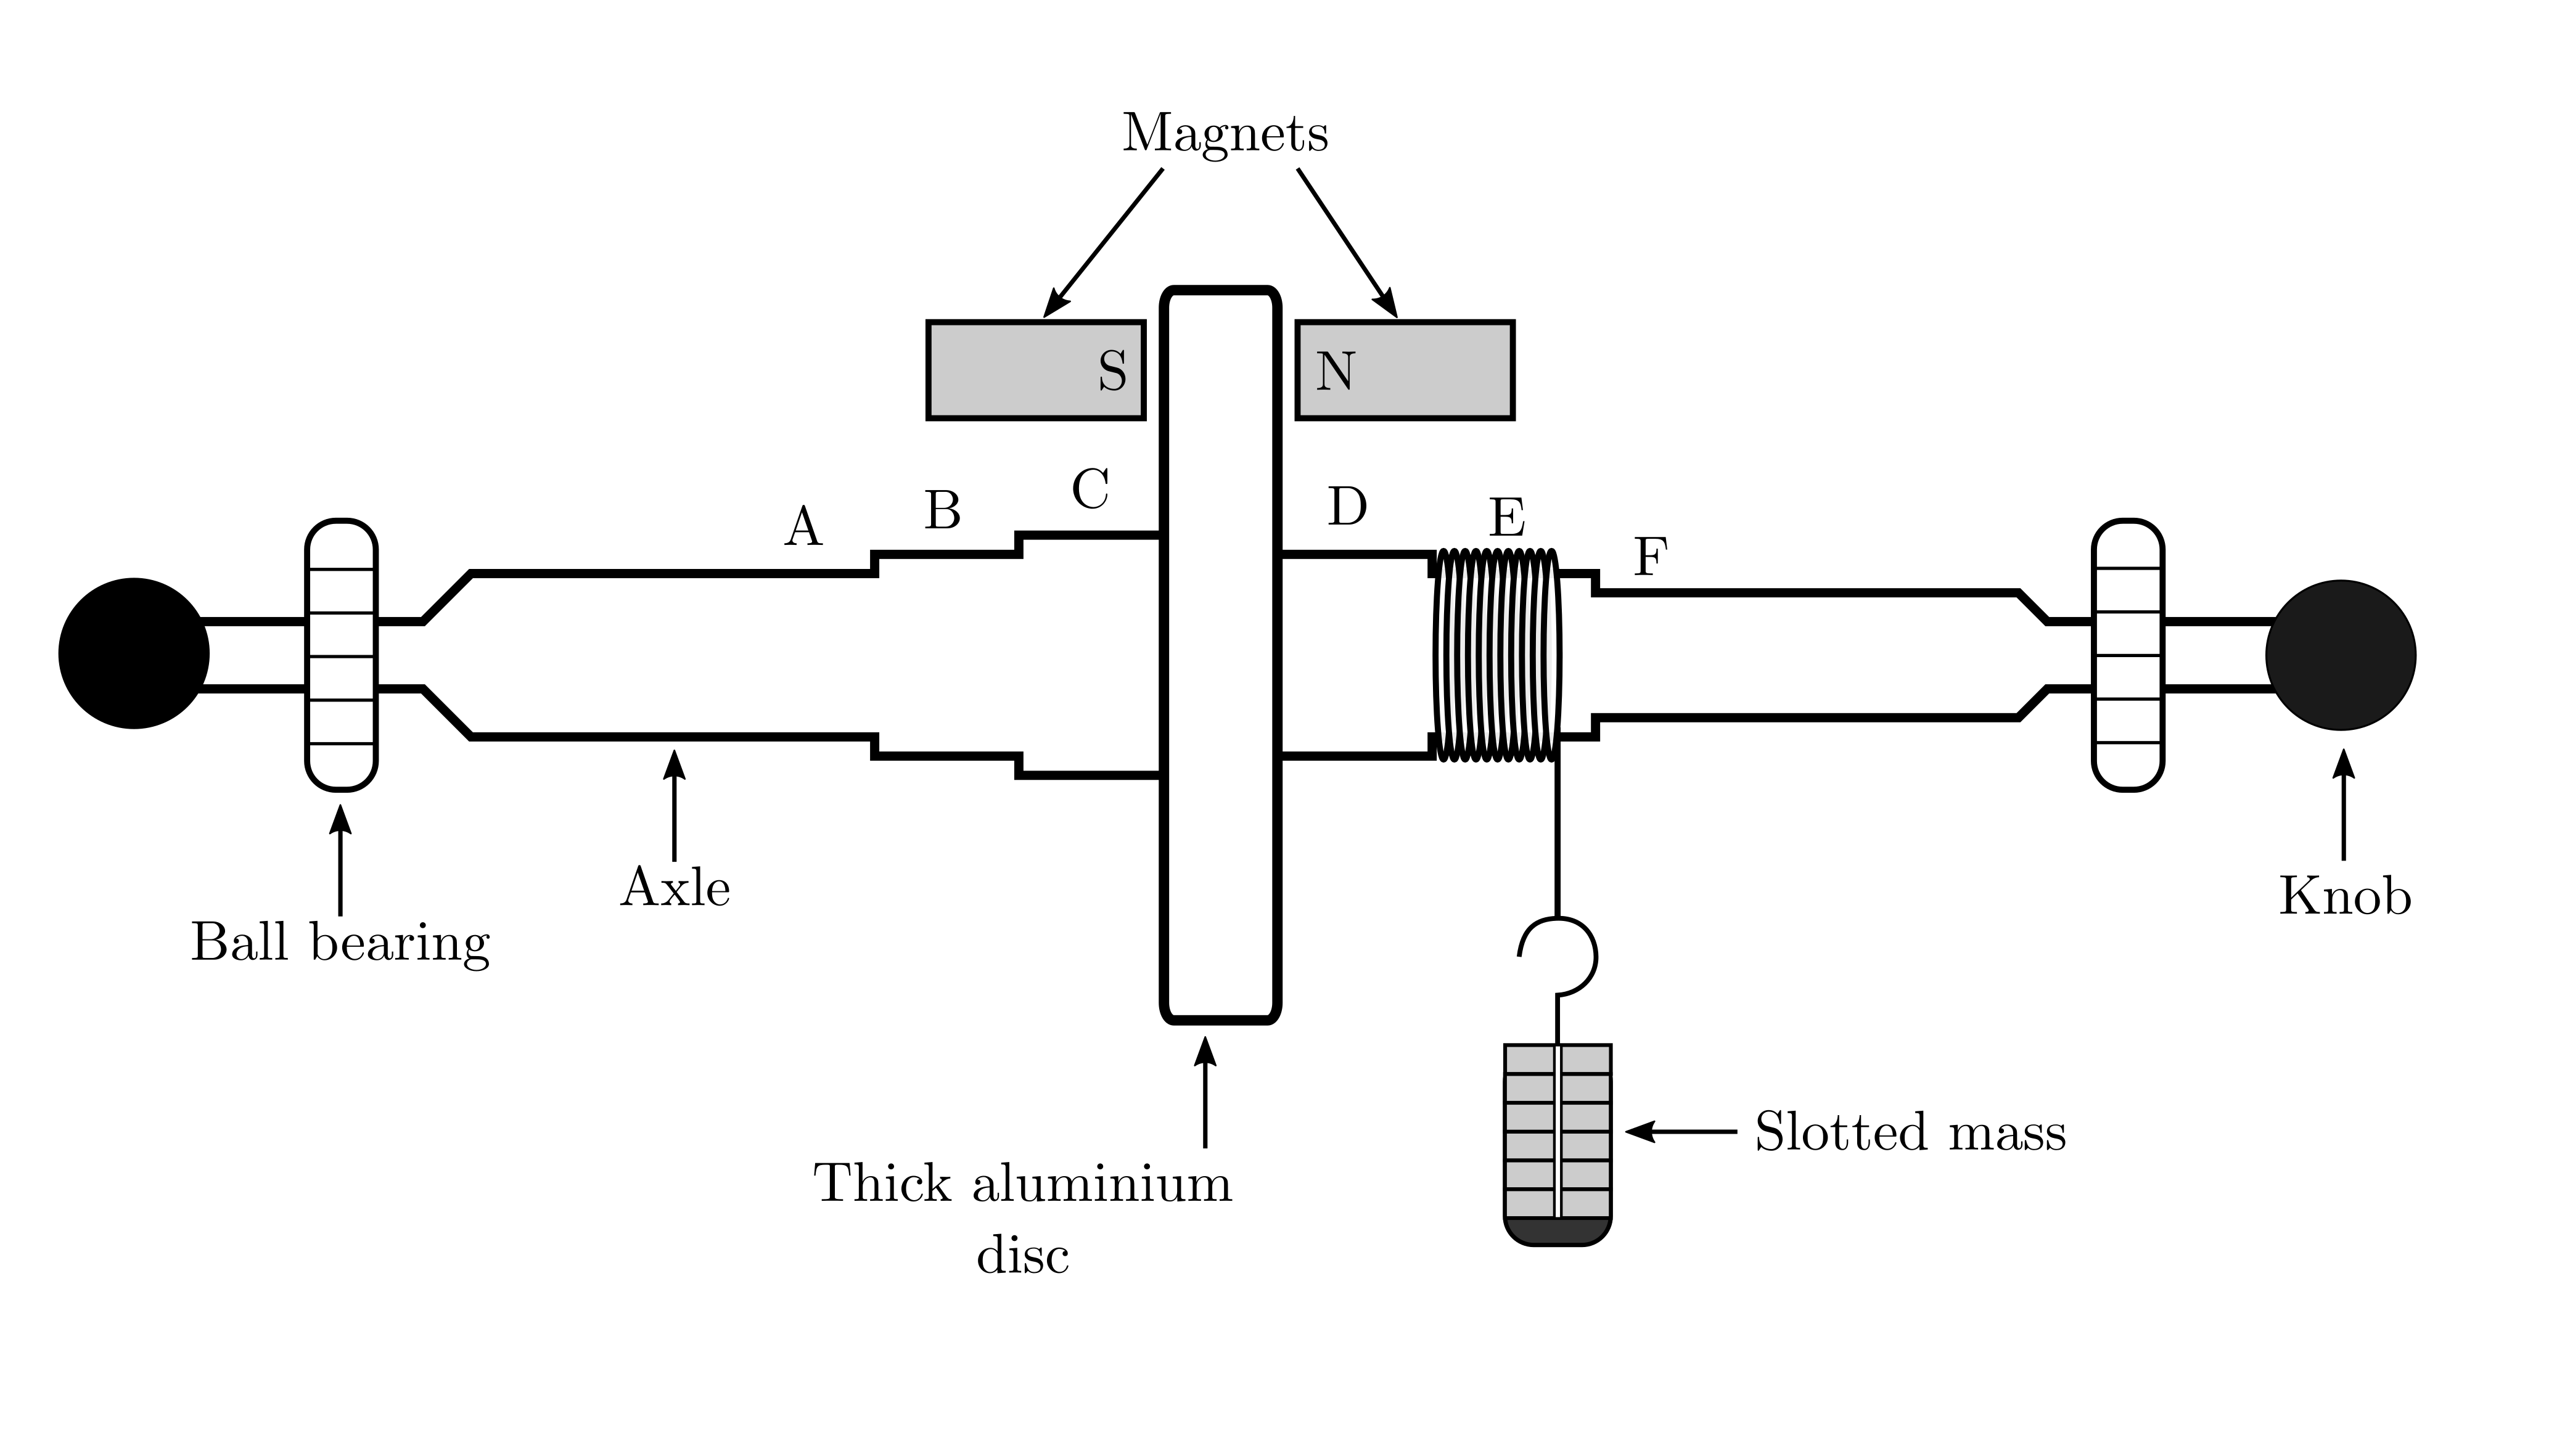
\includegraphics[width=\textwidth]{figs/em-damping/emdamping-setup.png}
    \caption{Schematic of the disc and magnet assembly. The different axles ($A$--$F$) are distinguished by their radii. The two magnets are placed on either side of the disc. The disc eventually rotates at a constant angular velocity because of the damping force due to the magnets. As a result, the slotted mass begins to fall with a constant terminal velocity.}
    \label{fig:emdamping-setup}
\end{figure}


\section*{Theory}

For rotating objects, Newton's Second Law may be generalised to 
\begin{equation}
    \tau = I \alpha
\end{equation}

where $\tau$ is the net external torque on the object, $I$ its moment of inertia, and $\alpha$ the angular acceleration. As the mass begins to fall, it will to accelerate, spinning the disk. It experiences two forces: gravity and the tension $T$ from the string, and thus accelerates at a rate $a<g$,
\begin{equation}
    ma = mg - T \quad \implies \quad T = m (g-a).
    \label{eqn:tension}
\end{equation}

\begin{figure}[!htb]
    \centering
    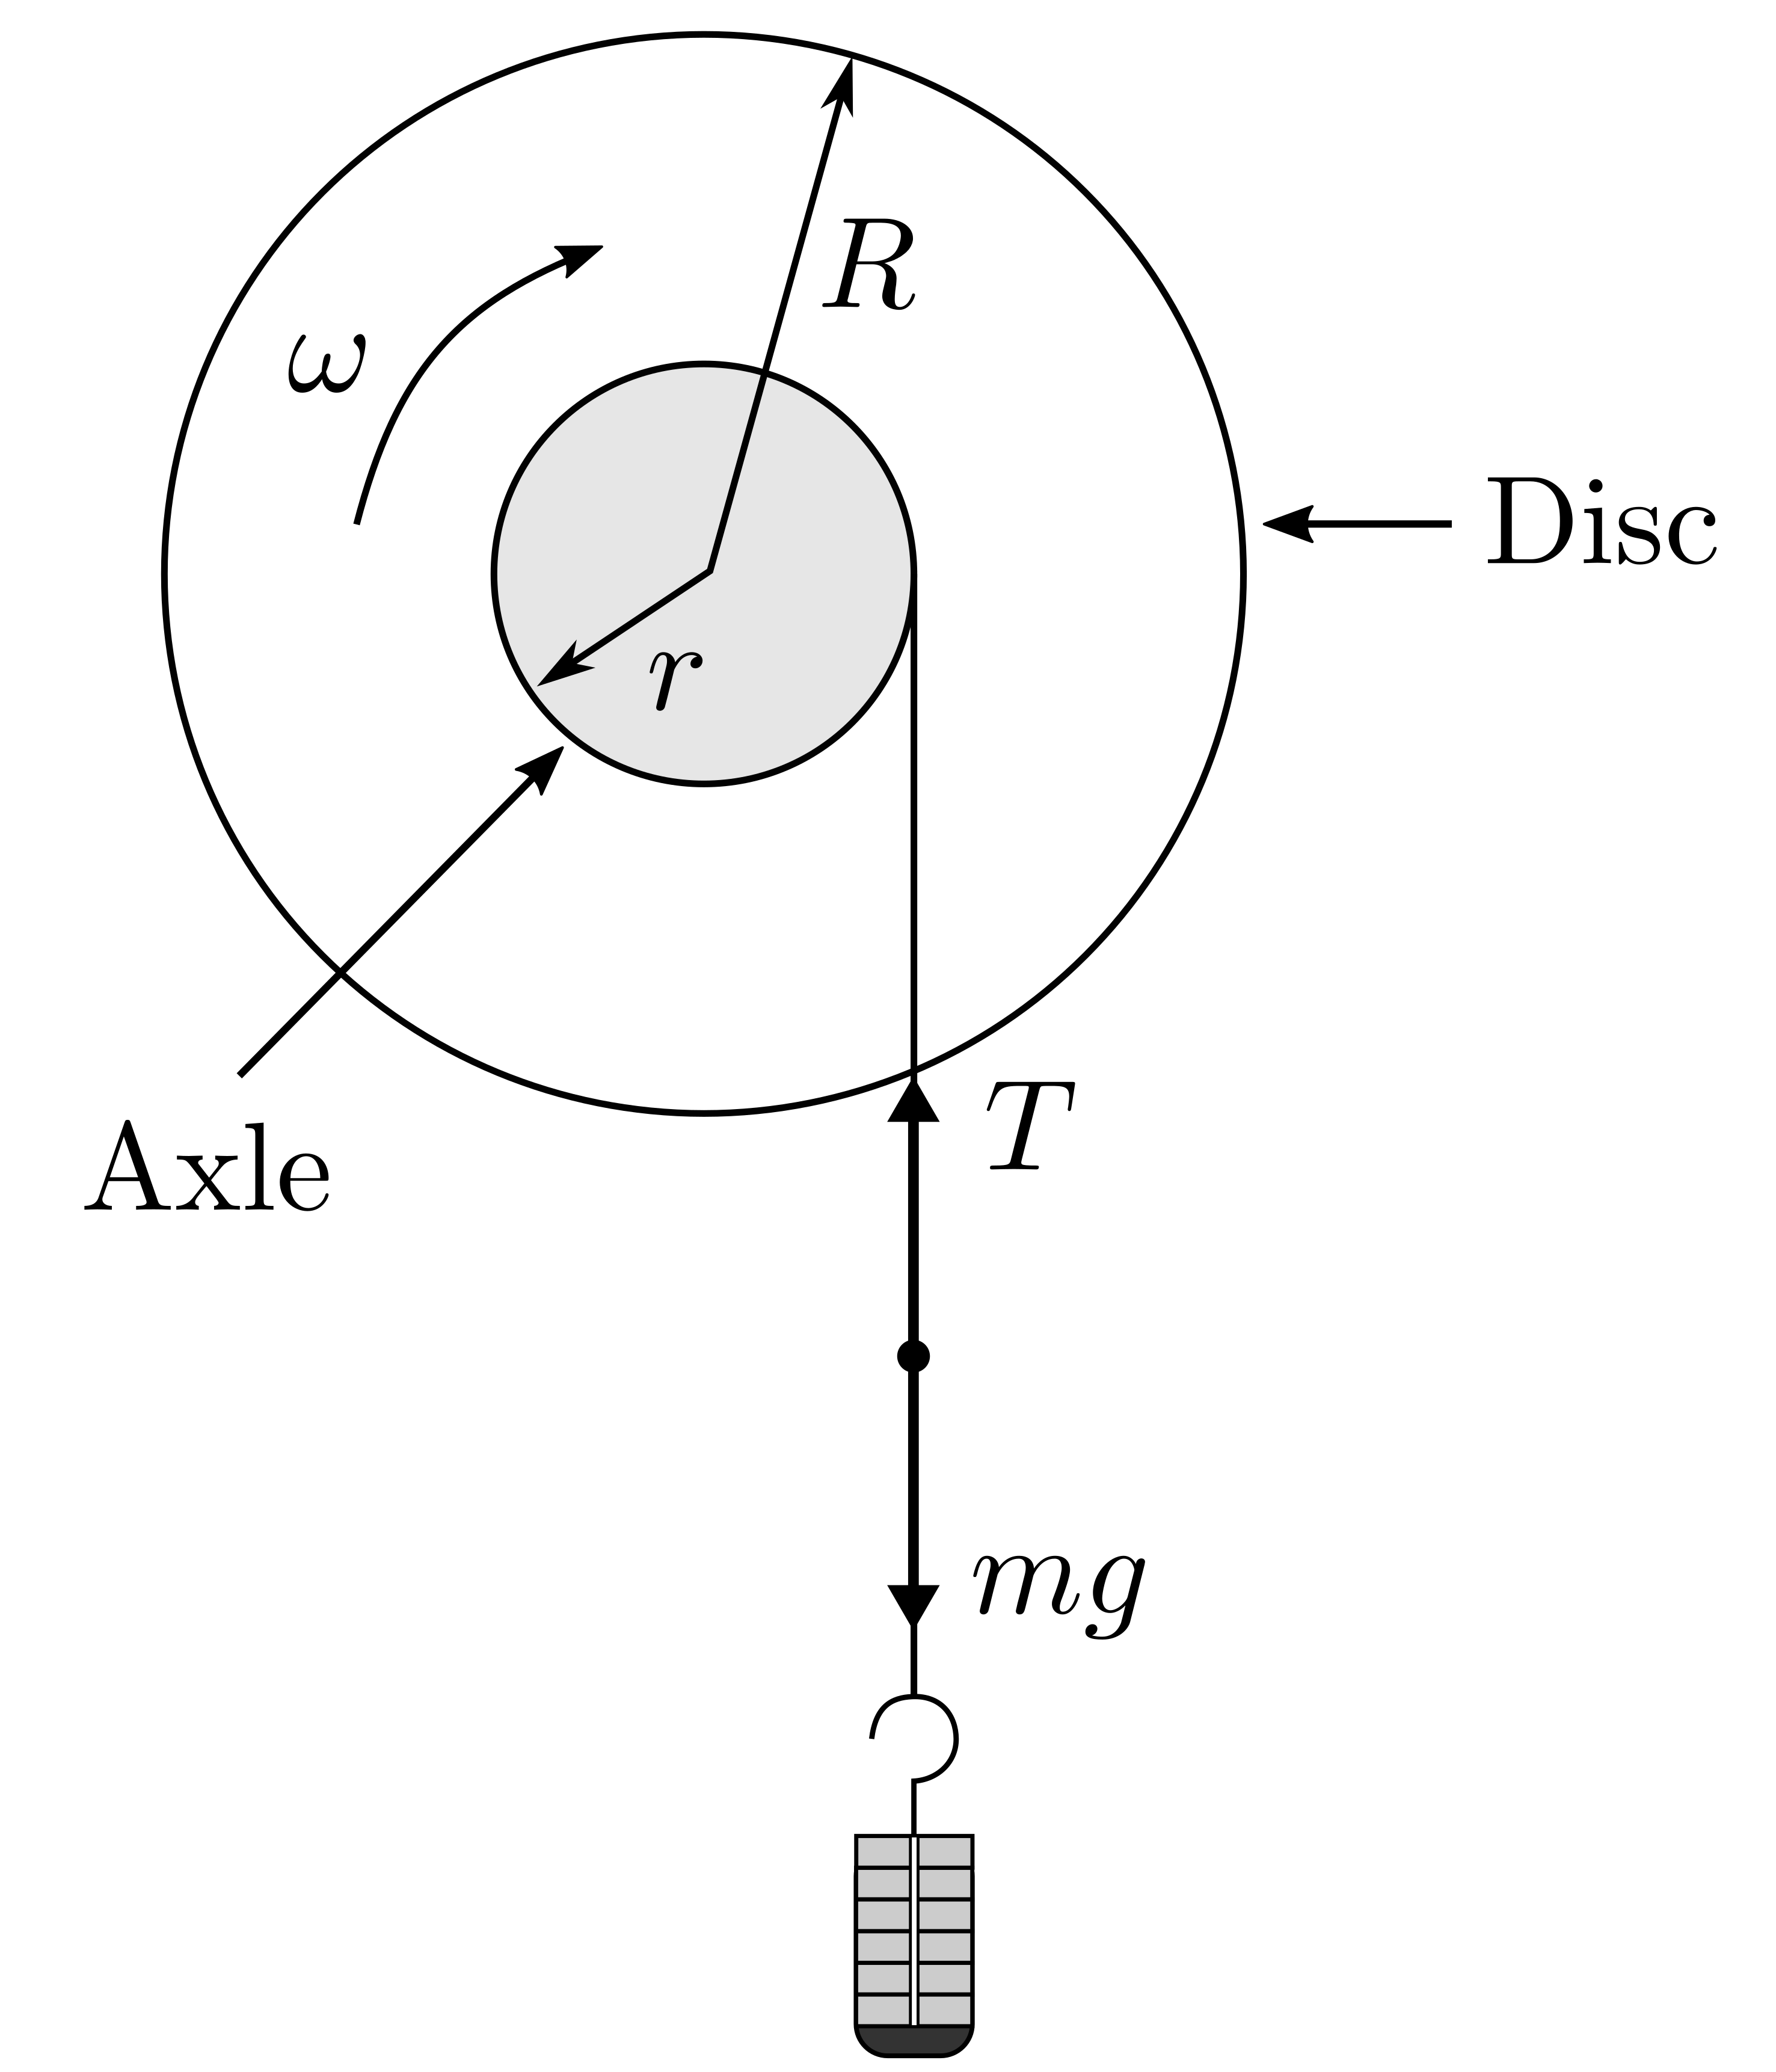
\includegraphics[width=0.4\textwidth]{figs/em-damping/emdamping-torque.png}
    \caption{View of the flywheel assembly from the side. The falling mass $m$ rotates the axle of radius $r$, which in turn causes the disc of radius $R$ to accelerate. Once the mass reaches terminal velocity due to electromagnetic damping, the disc moves at a constant angular velocity $\omega$. }
    \label{fig:emdamping-torque}
\end{figure}

Suppose the cord is wound around an axle of radius $r$. This means that the acceleration at the rim of the axle (i.e.\ at radius $r$) is the same as the acceleration of the mass. Thus
\begin{equation}
    \alpha = \frac{a}{r}
    \label{eqn:angularacc}
\end{equation}

\begin{question}
\textbf{Question:} The above situation is highly idealised, as it does not take into account friction. In practice, the disk will also experience a ``frictional'' torque $\tau_f$ which opposes its motion. Show, by balancing the torques on an axle of radius $r$, that 
\begin{equation}
    I \alpha = T r - \tau_f.
\end{equation}
\textbf{Question:} Using the equations for tension and angular acceleration (Equations~(\ref{eqn:tension}) and~(\ref{eqn:angularacc}) respectively) show that 
\begin{equation}
    a = g \left( \frac{m r^2}{I + mr^2}\right) - \left( \frac{r \tau_f}{I + mr^2}\right).
    \label{eqn:acc}
\end{equation}
\end{question}

\subsection*{Introducing damping}

The predominant damping in this set-up is due to electromagnetic damping. To understand how this occurs, let us focus on the electrons in the disc, which can move freely because the disc is a conductor. When an electron passes through the magnetic field, it experiences a Lorentz force $\vb{F} = e \vb{v} \times \vb{B}$. In this set-up, if we consider a point between the pole-pieces of the magnet, the magnetic field is perpendicular to the disc and the velocity of the electron is along the azimuthal direction. Thus the Lorentz force is along the radial direction. This force, acting on the electrons, causes them to systematically move in the radial direction. If the electrons were all pushed radially and could pile up at either the axle or the rim, an electric field would develop, which would grow until its effect exactly counteracted that of the magnetic field. But what we have here is a conductor that extends outward from the immediate vicinity of the pole pieces. Thus, the electrons moved by the Lorentz return to their original positions by a more circuitous route; closed, spread out currents are set up. Some of these eddy currents flow through the region between the pole pieces, and some of them flowing outside that region. 

Now let us focus on the current as it moves through the pole pieces. In these currents the charges move radially. A charge moving radially through the magnetic field experiences a force in the azimuthal direction. Note the three-step process: first, because the rotating conductor was carrying along the electrons with it, they were moving azimuthally, resulting in a radial Lorentz force; second, this radial Lorentz force causes a radial current, giving a radial component to the velocity of the electrons, and causing a current; third, the radially moving electrons in the current experience a Lorentz force in the azimuthal direction.

The question now arises: in which azimuthal direction does the Lorentz force on the radial current act? The direction can be established by carefully examining the direction of the field etc, but it can also be established from a more general principle. The azimuthal force must act such it it either helps the motion of the disk or hinders it. Suppose that the force acted such as to help the motion; then, a little push or fluctuation would start the process, and, with the help of the additional Lorentz force, would cause the wheel to turn faster, leading to a runaway situation that violates the conservation of energy. Thus the only possibility that can be realised in Nature is that the Lorentz force acts such as to hinder the motion of the wheel; it is a \textsl{damping} force.

Thus, the full torque balance on the disc is given by
\begin{equation}
    I \alpha = T r - \tau_f - \tau_B,
\end{equation}

where $\tau_B$ is the opposing magnetic torque that these currents produce. We will now try to calculate $\tau_B$ with an extremely simplified model.

\subsection*{Calculating the magnetic torque}

\begin{figure}[!htb]
    \centering
    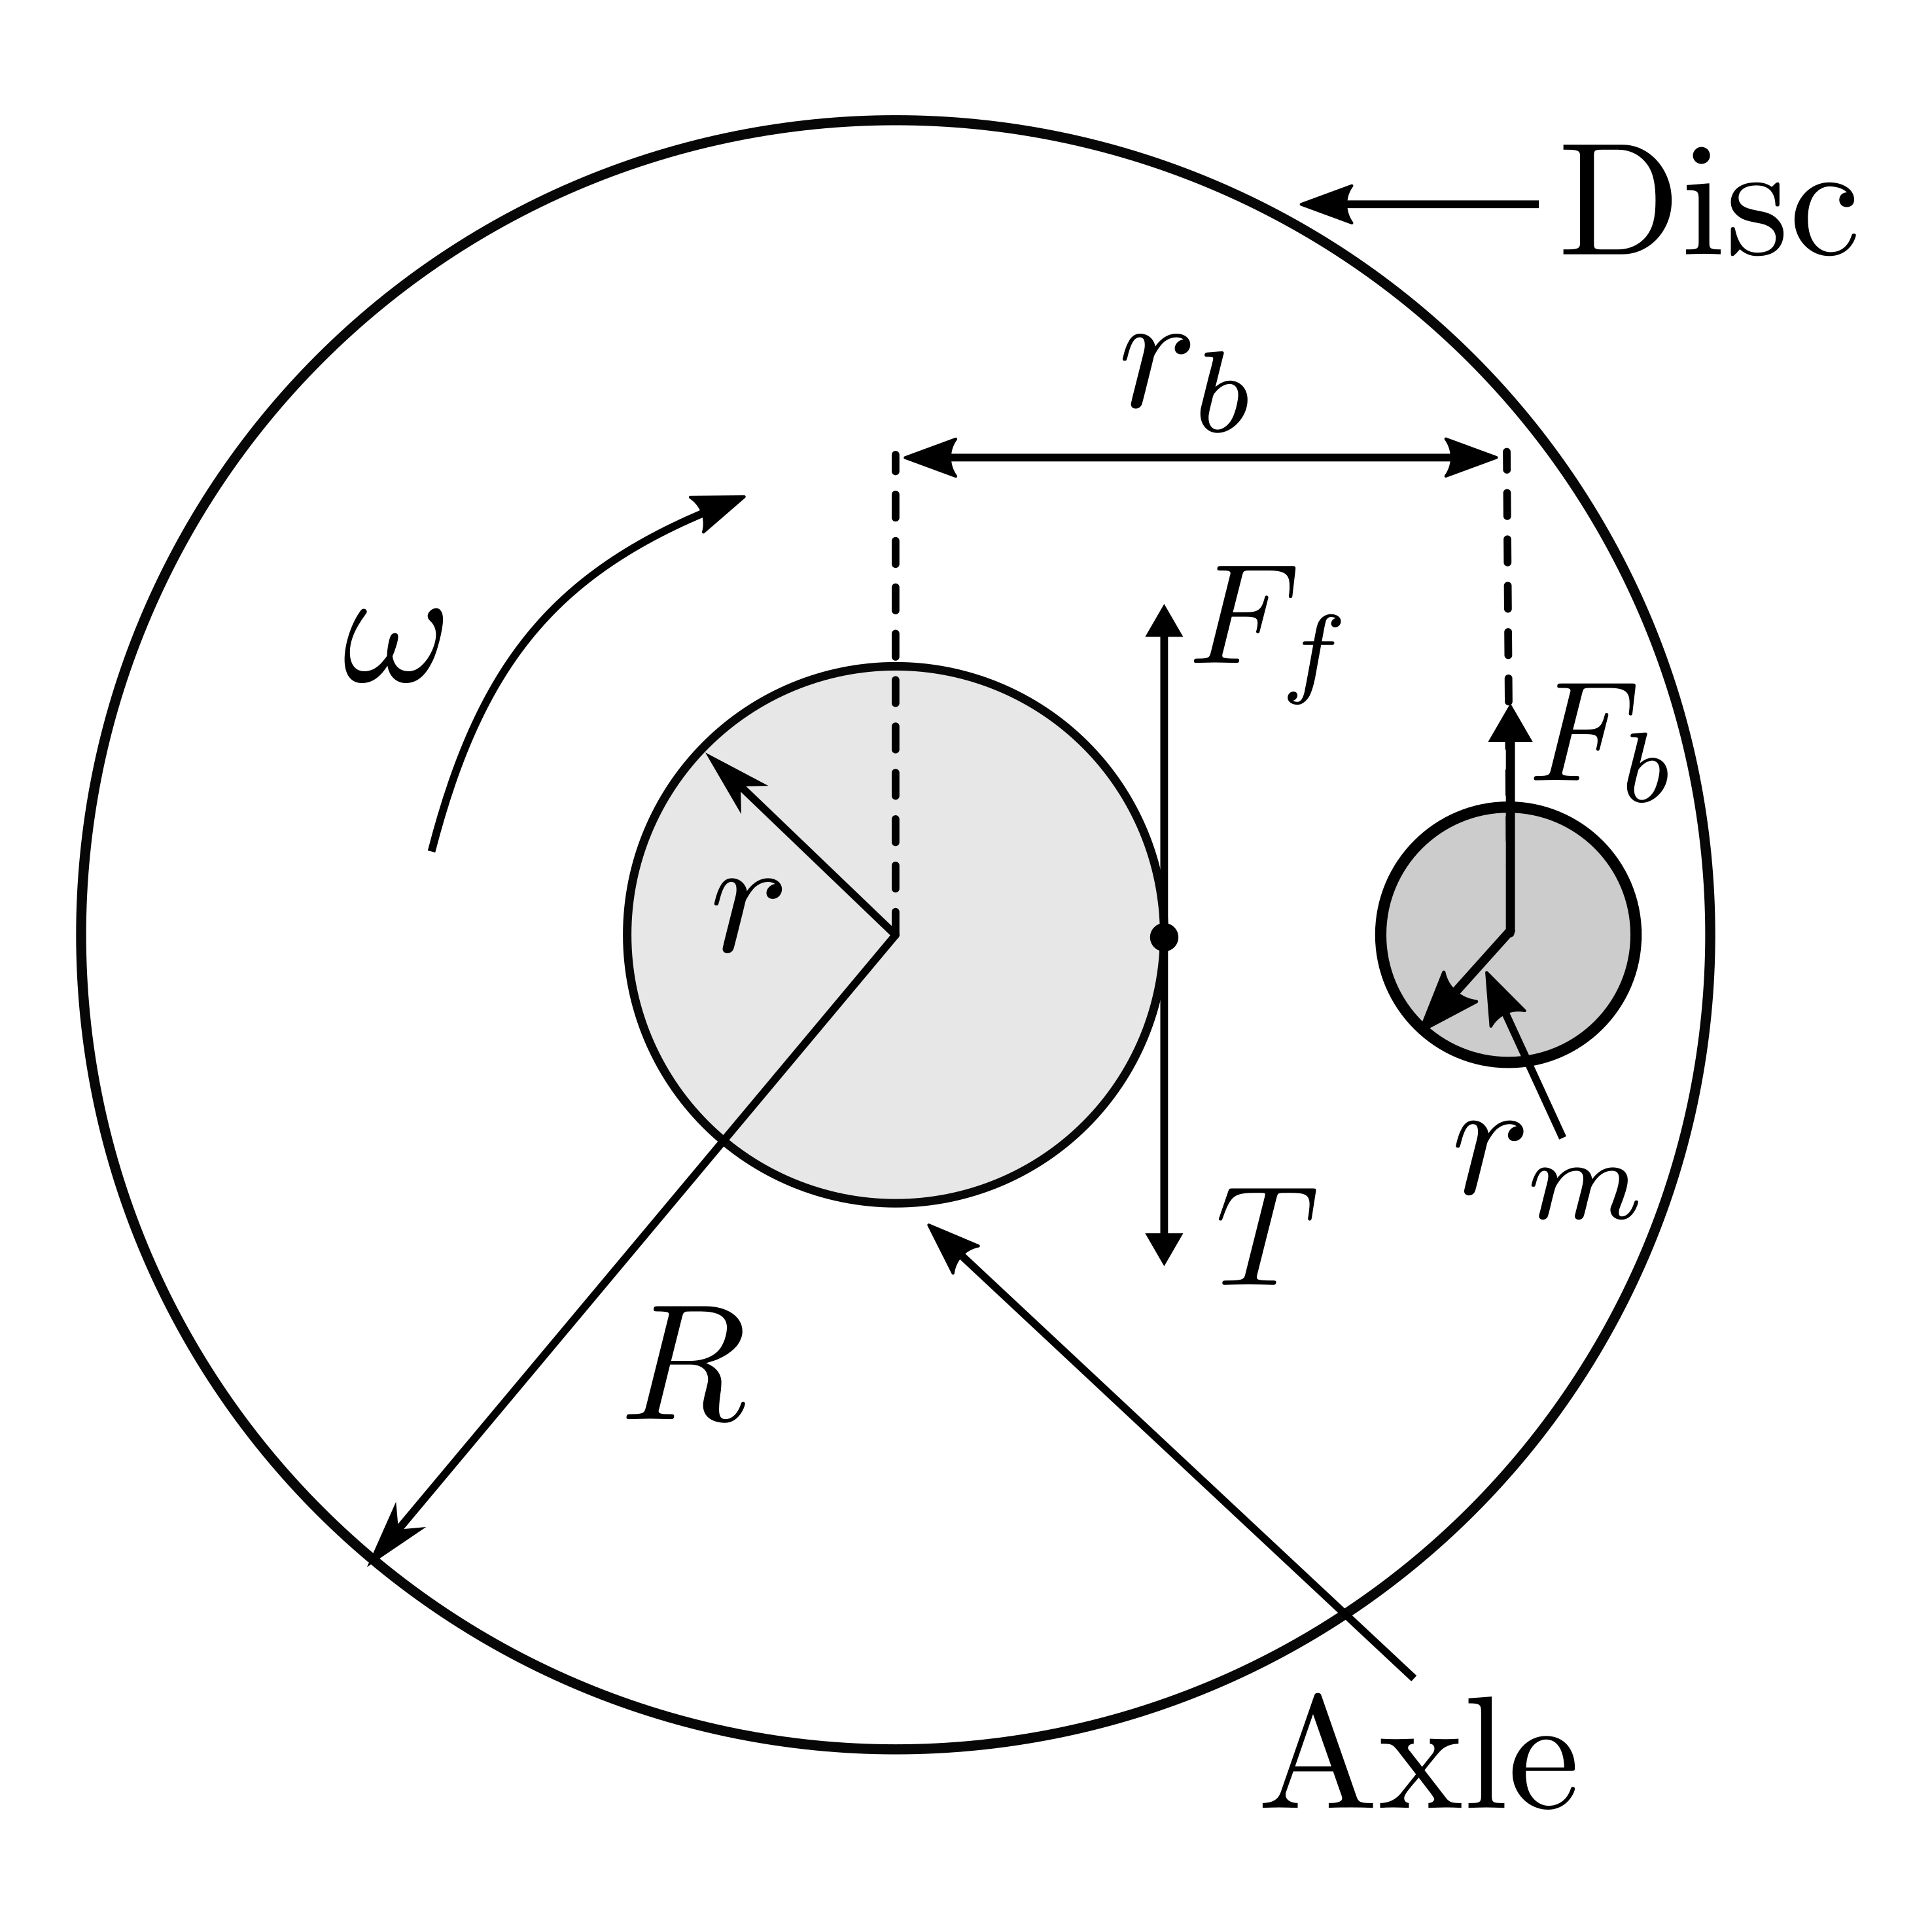
\includegraphics[width=0.4\textwidth]{figs/em-damping/emdamping-forces.png}
    \caption{View of the set-up from the side. The axle of the disc experiences a frictional force $F_f$ and the tension $T$ due to the string. A circular region of radius $r_m$, at a distance $r_b$ from the axle, experiences a damping force due to a nearly uniform $B$.}
    \label{fig:emdamping-forces}
\end{figure}

The magnetic field is confined to a small circular region $r_m \ll R$, the radius of the disc, as shown in Figure~(\ref{fig:emdamping-forces}), and is uniform over this region. Let us now consider a thin conducting path along the diameter of this region, of length $2 r_m$. It moves at a velocity $v = r_b \omega$, where $r_b$ is the distance from the centre of the circular region to the axis of rotation.

The emf $E_b$ induced is given by
\begin{equation}
    \mathcal{E}_b = (r_b \omega)\times B \times (2r_m).
\end{equation}

This emf $\mathcal{E}_b$ will give rise to a current $i$ (the eddy current) in a closed conducting path within the disc. Let us assume that this path has some resistance $R^*$.\footnote{This is a huge simplification: the reason eddy currents are so hard to model is because there are many different paths within the conductor of varying resistances.} Thus, the current is given by
\begin{equation}
    i = \frac{\mathcal{E}_b}{R^*} = \frac{(r_b \omega)\times B \times (2r_m)}{R^*}.
\end{equation}

These currents will in turn experience a force $F_b$ given by
\begin{equation}
    F_b = B i (2 r_m) = \frac{4 r_m^2 (\omega) r_b B^2}{R^*} = \left( \frac{4 r_m^2 r_b}{R^*}\right) \omega B^2.
\end{equation}

This force is responsible for the magnetic torque at $r$, $\tau_B$,
\begin{equation}
    \tau_B = r_b F_b = \left(\frac{4 r_m^2 r_b^2}{R^*} \right) \omega B^2 = C' \omega B^2.
\end{equation}

Now, in this derivation, we considered a conducting path going through the circular region of radius $r_m$. However, not all paths will have this length or even be radially directed. The effect of taking all these paths into consideration would be to given an average factor $C$ instead of $C'$. However, the dependence on $\omega$ and $B$ will remain unchanged. Thus, we can write the total torque as 
\begin{equation}
    I\alpha = m (g-a) r - \tau_f - C \omega B^2.
\end{equation}
As the retarding torque depends proportionately on the angular velocity of the disc, the disc will begin to slow until a steady state is obtained, i.e.\ until $\omega$ reaches some constant ``terminal'' value $\omega_t$. As a result, the mass will drop at some constant terminal velocity $v_t$. In this case, $\alpha=0$ and $a = 0$. 

\begin{question}
\textbf{Question:} Show that 
\begin{equation}
    v_t = \omega_t r = \left( \frac{g r^2}{CB^2}\right)\left( m - \frac{\tau_f}{g r}\right).
    \label{eqn:em-terminal}
\end{equation}
\end{question}

In this experiment, we will study the terminal velocity of the falling mass and its dependence on the mass and magnetic field.
 
\section*{Experimental Setup}


\subsection*{Apparatus}

\begin{enumerate}
\itemsep0em
\item A flywheel disc assembly, mounted on the wall
\item Two pairs of magnets with different pole strengths
\item A Gauss meter to measure magnetic fields
\item A set of slotted masses
\item A set of acrylic plates of different thicknesses
\item Metre scales and tapes
\item A spirit level
\end{enumerate}



% \subsection*{Description}


\subsection*{Precautions}
\begin{itemize}
\itemsep0em
\item Make sure the mass falls vertically, without horizontal oscillations.
\item The knobs on either end of the disc should be used to wind or unwind the cord.
\item Wind the cord on the axle carefully, so that the turns do not cross or overlap. Successive turns should touch each other, and should not extend beyond the length or diameter of the axle.
\end{itemize}



\section*{Procedure}

\subsection*{Part A}

You will begin this experiment by verifying Equation~(\ref{eqn:acc}) for the acceleration of the falling mass in the absence of a magnetic field. You will then use it determine the moment of inertia of the flywheel.

\begin{enumerate}
    \item Choose an appropriate axle and measure its diameter and note it down. Choose an appropriate length of cord and attach it to the axle.
    
    \item Attach the cord to a small slotted mass, and wind it carefully on the axle.
    
    \item Allow the mass to drop gently, taking care that it does not oscillate as it falls.
    
    \item Use a camera to take a video of the falling mass and analyse it to find its acceleration. You can use \textsl{Tracker} to obtain the position of the mass at different instants of time in the video.
    
    \item Once you have analysed your data for one video, repeat this procedure for different masses. 
    
    \item Plot an appropriate graph between the $a$ and $m$, and calculate the moment of inertia and frictional torque of the disc.
    
    % \begin{question}
    % \textbf{Question:} You will find that you have to plot a graph of the form
    % \begin{equation*}
    %     y = \frac{\alpha x}{\beta + x}
    % \end{equation*}
    
    % Show that by making a substitution $Y = 1/y$ and $X = 1/x$, you can reduce this graph to a linear graph
    
    % \begin{equation}
    %     Y = m X + C
    % \end{equation}
    
    % What are $m$ and $C$ in terms of $\alpha$ and $\beta$?
    % \end{question}
    \vspace{\parskip}
    \begin{question}
    \textbf{Question:} You will find that you have to plot a graph of the form
    \begin{equation*}
        a =  g \left( \frac{m r^2}{I + mr^2}\right) - \left( \frac{\tau_f r}{I + mr^2}\right)
    \end{equation*}
    
    Show, using an appropriate approximation, that this relation reduces to:
    
    \begin{equation}
        a \approx m \left( \frac{g r^2}{I}\right) - \left( \frac{\tau_f r}{I}\right).
    \end{equation}
    
    How would you find $I$ and $\tau_f$?
    \end{question}
    
\end{enumerate}

% \begin{question}
% \textbf{Question:} Would y-intercept would you expect this graph to have?
% \begin{enumerate}
%     \item Positive
%     \item Zero
%     \item Negative
% \end{enumerate}

% What do you think is responsible for this intercept?
% \end{question}

\subsection*{Part B}

Next, you will introduce electromagnetic damping to this system, which will make the mass fall at a terminal velocity $v_t$.
\begin{enumerate}
    \item Insert a pair of magnets in their holders, and place them on the assembly.
    
    \item Make sure that the magnets are equally spaced from the disc. In order to do this, bring them as close to the disc as possible, and note down the readings on the screw gauges on either side. Using this as your reference, rotate the screw gauge by the same amount on either side.
    
    \item Repeat the procedure given in \textbf{Part A}. In this case, the disc should finish by rotating at a constant angular velocity due to the electromagnetic damping.
    
    \item Plot a graph between the terminal velocity and the mass of the object, and show that it satisfies the relation for the terminal velocity given in Equation~(\ref{eqn:em-terminal}).
    
\end{enumerate}

\subsection*{Part C}

Finally, you will vary the strength of the magnetic field and measure how the terminal velocity $v_t$ varies with the external magnetic field $B$.
\begin{enumerate}
    \item Vary the distances between the magnets and measure the magnetic field $B$ exactly between the magnets using a Gauss meter. Plot a graph of $B$ as you vary the magnets' separation. This graph will tell you what the magnetic field should be at the centre of the disk as you vary the separation between the magnets.
    
    \item Next, keep the magnets some known distance apart and measure $v_t$ for a fixed value of mass. 
    
    \item Without changing any of the parameters in the system (including the mass), change the separation between the magnets (effectively varying $B$) and calculate the $v_t$. Repeat this for different separations between the magnets. Find how the terminal velocity $v_t$ varies with $B$.
    
\end{enumerate}